\documentclass{article}
\usepackage{microtype}
\usepackage{graphicx}
\usepackage{booktabs}
\usepackage{xurl}
\usepackage{hyperref}
\usepackage{icml2026}
\usepackage{amsmath,amssymb,amsthm,mathtools}
\usepackage[capitalize,noabbrev]{cleveref}
\newtheorem{theorem}{Theorem}
\newtheorem{proposition}[theorem]{Proposition}
\newtheorem{corollary}[theorem]{Corollary}
\newtheorem{lemma}[theorem]{Lemma}
\newcommand{\PP}{\mathbb P}
\newcommand{\EE}{\mathbb E}
\newcommand{\ind}{\mathbf 1}
\newcommand{\R}{\mathbb R}
\newcommand{\Cov}{\operatorname{Cov}}
\newcommand{\ranknet}{N_{\mathrm{rank}}}
\newcommand{\SevereMean}{0.8863}
\newcommand{\SevereTheory}{0.8866}
\newcommand{\SevereCI}{0.0006}
\newcommand{\SevereFixed}{89.9700}
\newcommand{\SevereSplit}{90.1919}
\newcommand{\NumOccupancyCases}{21}
\newcommand{\RunSeconds}{10.88}

\makeatletter
\newcommand{\inputtable}[1]{\@@input#1 }
\makeatother
\icmltitlerunning{Limits of Smooth Scalar Tuning in Split Conformal Prediction}
% Local draft notice only. Restore the official notice for a real submission.
\makeatletter
\renewcommand{\Notice@String}{Local research draft, September 28, 2026. Not submitted. Uses the ICML 2026 template provisionally.}
\makeatother
\hypersetup{pdftitle={Limits of Smooth Scalar Tuning in Split Conformal Prediction},pdfsubject={Local research draft},pdfauthor={}}
\begin{document}
\twocolumn[
\icmltitle{Limits of Smooth Scalar Tuning in Split Conformal Prediction}
\begin{icmlauthorlist}
\icmlauthor{Anonymous Authors}{anon}
\end{icmlauthorlist}
\icmlaffiliation{anon}{Anonymous Institution}
\icmlcorrespondingauthor{Anonymous Author}{anon.email@domain.com}
\icmlkeywords{conformal prediction, calibration, model selection, statistical complexity}
\vskip 0.3in
]
\printAffiliationsAndNotice{}

\begin{abstract}
Reusing calibration data to tune a conformal score can reduce coverage. Does tuning a single smooth parameter make this effect small? We construct a compact scalar family of bounded, infinitely differentiable, 1-Lipschitz scores with continuous score distributions for which ordinary recalibration has arbitrarily small finite-sample coverage. The construction encodes label subsets and gives an exact occupancy formula; it requires increasing parameter precision, so it is a worst-case result rather than a model of ordinary temperature scaling. At nominal 90\% coverage, a specified case gives \SevereMean\% in 10,000 calibration repetitions, versus \SevereTheory\% analytically. We express a sufficient condition through covering numbers of population-transformed scores, using classical beta order statistics. Raw-score Lipschitzness transfers to this condition when combined with anti-concentration. We also explain how classical uniform convergence ensures consistency of each fixed compact atomless continuous family, despite the absence of a uniform dimension-only rate. The contribution clarifies the assumptions behind adaptive calibration guarantees; it does not introduce a practical replacement for valid post-selection methods.
\end{abstract}

\section{Introduction}

Split conformal prediction converts a score into a prediction set using a calibration order statistic. Its finite-sample guarantee applies when the score is fixed independently of the calibration data. Choosing the score using those same observations changes the problem: the selected order statistic can be systematically optimistic. This is an established model-selection issue, with existing remedies and quantitative bounds \citep{yang2025,liang2026}.

A tempting justification for data reuse is that only a small number of parameters are tuned. Statistical complexity, however, belongs to the induced functions and decisions, not to the number of coordinates used to describe them. Even a scalar may index many different orderings. Smoothness of the raw score also needs interpretation: multiplying every score by a small positive constant decreases its Lipschitz constant without changing any conformal prediction set.

This distinction is relevant to a specific published argument. \citet{zeng2025} propose a parameter-dimensional bound on tuning bias. In their published appendix, Lemmas D.3 and D.5 infer bounds on the VC dimension of score sublevel sets from bounded continuity in the parameters. That implication is not valid in general. Our construction gives an explicit counterexample satisfying stronger smoothness assumptions. This observation concerns the general argument; it does not challenge the numerical measurements for the particular calibrators evaluated in that work.

The general possibility of severe adaptive failure is already known. For example, \citet{crc2024} show that conformal risk control can fail arbitrarily badly for non-monotone losses. Our question is narrower: what happens when a \emph{smooth score family} is selected and then recalibrated by an ordinary split-conformal quantile, with no ties in any fixed score distribution? We obtain an exact answer for a finite-label construction, and connect it to conditions sufficient for consistency.

The resulting contributions are:
\begin{enumerate}
\item A compact, smooth, 1-Lipschitz scalar construction with exact coverage $c_n[1-(1-1/K)^n]$, where $c_n$ is fixed-score conformal coverage and $K$ is the label-universe size.
\item An exponential lower bound on a covering number of its population score ranks, showing why the raw Lipschitz bound hides substantial complexity.
\item A beta-tail covering certificate that makes the score scale irrelevant, together with an explicit connection to classical fixed-family consistency. The latter is a standard consequence of uniform laws of large numbers, not a new consistency theorem.
\end{enumerate}

The examples are intentionally constructed. In particular, one scalar encodes $2^K$ alternatives, and large-$K$ evaluation uses an equivalent exact mask representation. The paper establishes a limit on universal guarantees, not a prevalence claim about modern neural-network tuning.

\section{Related Work}

\paragraph{Conformal selection.}
\citet{yang2025} analyze efficiency-first selection using finite-family empirical-process bounds and validity-first selection using another split. \citet{liang2026} develop valid procedures that incorporate model selection into the conformal construction. Their efficiency analysis uses class complexity and regularity. We study the unmodified reused-calibration rule; we do not claim that it outperforms their valid procedures. The finite-family part of our certificate is closely related to these bounds.

\paragraph{Conditional validity and complexity.}
The fixed-score binomial and beta order-statistic analysis is classical in conformal inference \citep{vovk2012}. Covering numbers and anti-concentration also appear together in \citet{kiyani2024}, who study learned prediction-set thresholds under conditional-coverage requirements. Our certificate instead covers population-transformed \emph{scores}, applies to an arbitrary measurable selector, and makes invariance to increasing score transformations explicit. It requires population information and is not an estimated certificate. Qualitative consistency is already implied by compact-parameter uniform laws of large numbers, such as \citet[Lemma 2.4]{newey1994}; we state the connection to delimit the counterexample, not as a separate novelty claim.

\paragraph{Non-monotone risk control.}
The counterexample in \citet{crc2024} already rules out unrestricted non-monotone scalar tuning. Recent preprints study stability-based guarantees \citep{angelopoulos2026} and finite-grid behavior \citep{aldirawi2026}. Smoothness of a real-valued score does not imply smoothness of the thresholded miscoverage loss; thus our example does not contradict results that impose regularity on the \emph{loss} or stability on the selector. The exact occupancy law and its compatibility with smooth atomless scores are the distinctions pursued here. A full closest-work matrix and version-specific reading record accompany the manuscript.

\section{Setup}

Let $Z_i=(X_i,Y_i)$, $i=1,\ldots,n+1$, be i.i.d. from $P$. The score family $\{S_\lambda:\lambda\in\Lambda\}$ is fixed before observing $D=(Z_1,\ldots,Z_n)$; independently trained models may be conditioned on. Write
\begin{equation}
 k=\lceil(n+1)(1-\alpha)\rceil,\qquad c_n=\frac{k}{n+1}.
\end{equation}
For $k\le n$, let $q_\lambda$ be the $k$th order statistic of the calibration scores and define
\begin{equation}
 C_D(x)=\{y:S_{\hat\lambda(D)}(x,y)\le q_{\hat\lambda(D)}\}.
\end{equation}
The selector $\hat\lambda$ may use all calibration observations but not the test observation. It is measurable. Let $F_\lambda$ denote the population CDF of $S_\lambda(Z)$ and write the calibration-conditional coverage as
\begin{equation}\label{eq:conditional}
 V_D=\PP\{Y_{n+1}\in C_D(X_{n+1})\mid D\}
     =F_{\hat\lambda}(q_{\hat\lambda}).
\end{equation}
Marginal coverage is $\EE V_D$. For every fixed $\lambda$ with continuous $F_\lambda$, $F_\lambda(q_\lambda)$ has the $\operatorname{Beta}(k,n+1-k)$ distribution and expectation $c_n$. If $k=n+1$, the conformal threshold is $+\infty$ and coverage is one; results involving finite beta parameters below concern $k\le n$.

\section{A Smooth Scalar Counterexample}

Take $X=U\sim\operatorname{Unif}[0,1]$ independently of $Y\sim\operatorname{Unif}\{0,\ldots,K-1\}$. Let $M=2^K$ and enumerate subsets $A_j$ by binary masks $j=0,\ldots,M-1$. Their scalar locations are $\lambda_j=j/(M-1)$. At these locations, we want scores
\begin{equation}\label{eq:knots}
 \begin{aligned}
 S_{\lambda_j}(u,y)&=a_K\left(\ind\{y\notin A_j\}+\frac{u}{4}\right),\\
 a_K&=\frac{1}{8(M-1)}.
 \end{aligned}
\end{equation}
The common positive factor $a_K$ affects neither score rankings nor prediction sets.

To interpolate, define $\psi(t)=e^{-1/t}$ for $t>0$, zero otherwise, and
\begin{equation}\label{eq:smooth}
 h(t)=\frac{\psi(t)}{\psi(t)+\psi(1-t)}.
\end{equation}
On $[\lambda_j,\lambda_{j+1}]$, interpolate the two membership indicators with weight $h((M-1)\lambda-j)$ and add $u/4$, all multiplied by $a_K$. Extend constantly beyond the endpoint knots. The function is infinitely differentiable because $h$ is flat at zero and one. Moreover, $0\le h\le1$ and $\sup|h'|\le8$ (Appendix~\ref{app:smooth}). Thus $S_\lambda\in[0,1]$ and $|S_\lambda(z)-S_\mu(z)|\le|\lambda-\mu|$. At every parameter, the uniform $U$ term gives an atomless score distribution.

\begin{theorem}[Exact occupancy coverage]\label{thm:occupancy}
For any $n,K\ge1$ and $\alpha\in(0,1)$ with $k\le n$, the above smooth scalar family and the selector choosing the knot for
\begin{equation}
 A(D)=\{Y_1,\ldots,Y_n\}
\end{equation}
satisfy
\begin{align}
 V_D&=\frac{|A(D)|}{K}U_{(k)},\label{eq:conditional-occupancy}\\
 \EE V_D&=c_n\left[1-\left(1-\frac1K\right)^n\right].\label{eq:occupancy}
\end{align}
Every fixed member of the family instead has marginal coverage $c_n$.
\end{theorem}

\begin{proof}
Every calibration label belongs to $A(D)$, so its selected score is $a_KU_i/4$ and the threshold is $a_KU_{(k)}/4$. A future label outside $A(D)$ has score at least $a_K$ and cannot be included. A label inside is included exactly when $U\le U_{(k)}$. This proves \cref{eq:conditional-occupancy}. The set $A(D)$ depends only on the labels and is independent of all $U_i$. Each of the $K$ labels is observed with probability $1-(1-1/K)^n$, while $\EE U_{(k)}=c_n$. Multiplying expectations proves \cref{eq:occupancy}. Fixed-score validity follows from its continuous score distribution.
\end{proof}

The selector can be expressed as minimizing a fixed loss, rather than specifying an adaptive score family. At the knots, minimize the number of calibration labels excluded from $A$ plus $|A|/(K+1)$; assign infinite loss away from the knots. Including an observed label decreases this loss, and including an unobserved label increases it. Thus its unique minimizer is $A(D)$. The loss itself is not assumed continuous; this is an unrestricted measurable selection result, not a claim about gradient descent.

\paragraph{What fails uniformly.}
By $1-(1-1/K)^n\le n/K$, the marginal coverage is at most $c_nn/K$ and can be made arbitrarily small for each fixed $n$ with $k\le n$. The coverage decrease relative to the fixed-score baseline equals
\begin{equation}\label{eq:reuse}
 c_n-\EE V_D=c_n(1-1/K)^n.
\end{equation}
Consequently no vanishing finite-sample bound depending only on $n$, scalar dimension, the common Lipschitz bound and the common score range can hold uniformly over these families. Choosing a large $n$ and then a sufficiently large $K$ defeats any universal $C/\sqrt n$ bound. This is a statement across families. For each \emph{fixed} $K$, \cref{eq:reuse} tends to zero.

\paragraph{What the scalar hides.}
The parameter distinguishes $2^K$ knots; representing all of them requires at least $K$ bits of distinguishability. The construction is neither a one-parameter computational shortcut nor a realistic model of temperature scaling. Ordinary finite precision restricts the available alternatives, to which finite-family guarantees apply. At $u=1/2$ and threshold $a_K/2$, the knots realize all $2^K$ subsets of the $K$ labels. Hence the threshold class has VC dimension at least $K$ despite bounded smooth scalar parameterization. Appendix~\ref{app:implementation} provides a direct three-label illustration.

\begin{figure*}[t]
\centering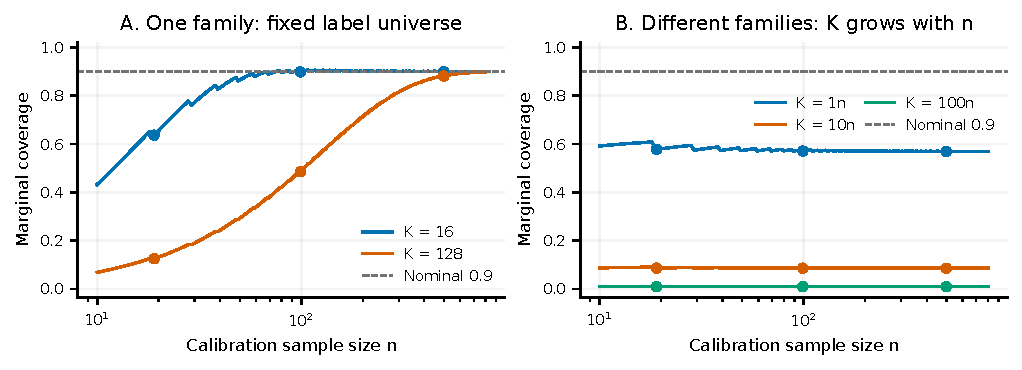
\includegraphics[width=\textwidth]{figures/occupancy.pdf}
\caption{Does the counterexample imply permanent inconsistency? Curves are exact coverage; points are means of 10,000 independent calibration samples with pointwise 95\% Monte Carlo intervals (often smaller than the markers). Left: a fixed family approaches nominal coverage. Right: choosing a different family as $K$ grows with $n$ preserves substantial loss. All large-$K$ computations evaluate the equivalent knot-mask event, not a floating-point encoding of the scalar.}
\label{fig:occupancy}
\end{figure*}

\section{Complexity on the Probability Scale}

For atomless score distributions define the population-transformed scores
\begin{equation}
 R_\lambda(z)=F_\lambda(S_\lambda(z))\in[0,1].
\end{equation}
Each $R_\lambda(Z)$ is uniform. Transforming a score by any strictly increasing function leaves $R_\lambda$ unchanged. This removes irrelevant raw-score scales from the analysis. Throughout, suprema over $z$ use a common domain on which the stated uniform bounds hold.

Let $\ranknet(r)$ be the smallest size of a deterministic set of parameter representatives such that every $R_\lambda$ is within $r$ in sup norm of a representative. The centers and radius must be fixed independently of the calibration sample. This population-dependent quantity is used for analysis, not estimated from the reused observations.

\begin{theorem}[Rank-cover certificate]\label{thm:net}
Suppose $\ranknet(r)\le N<\infty$. Write $B_{n,k}$ for the CDF of $\operatorname{Beta}(k,n+1-k)$. For every measurable selector and $u,v\in[0,1]$,
\begin{align}
 \PP\{V_D<u-r\}&\le N B_{n,k}(u),\label{eq:lower}\\
 \PP\{V_D>v+r\}&\le N[1-B_{n,k}(v)].\label{eq:upper}
\end{align}
In particular, for $\delta\in(0,1)$, with probability at least $1-\delta$ over $D$,
\begin{equation}\label{eq:certificate}
 V_D\ge\left[B_{n,k}^{-1}(\delta/N)-r\right]_+.
\end{equation}
\end{theorem}

\begin{proof}
Order statistics commute with nondecreasing transformations, so \cref{eq:conditional} is exactly the $k$th order statistic of $R_{\hat\lambda}(Z_i)$. If two arrays differ by at most $r$ coordinatewise, their $k$th order statistics differ by at most $r$. Therefore, with $T_j$ the order statistic for representative $j$,
\begin{equation}\label{eq:bracket}
 \min_{j\le N}T_j-r\le V_D\le\max_{j\le N}T_j+r.
\end{equation}
Each fixed $T_j$ has the beta law. Applying a union bound proves both tails; the representatives need not be independent. Inverting the lower-tail bound and using $V_D\ge0$ gives \cref{eq:certificate}.
\end{proof}

For $M$ fixed candidate scores, taking $r=0,N=M$ recovers an exact beta-tail union certificate. For a collection of strictly increasing transformations of one score, $N=1,r=0$: even data-dependent selection cannot change the prediction sets. This invariance is already explicit in \citet{zeng2025}, Lemma D.7. The new role here is its inclusion in the same complexity description as the adverse construction.

\begin{proposition}[Large rank covers in the construction]\label{prop:separation}
Let $K\ge2$, $m=\lfloor K/2\rfloor$ and $p=m/K$. For the family in \cref{thm:occupancy},
\begin{equation}
 \ranknet(r)\ge \binom{K}{m}\quad\text{whenever }r<p/2.
\end{equation}
\end{proposition}
\begin{proof}
Restrict to knots with $|A|=m$. Their transformed scores equal $pu$ when $y\in A$, and $p+(1-p)u$ otherwise. For two distinct subsets choose a label in their symmetric difference and let $u$ tend to zero. The sup-norm distance is at least $p$. A ball of radius $r<p/2$ cannot contain two such functions, so each requires a distinct cover element.
\end{proof}

Thus the rank covering complexity stays exponentially large in $K$ at a constant radius, even though raw scores have a common Lipschitz bound. Shrinking score amplitude does not remove the relevant statistical complexity.

\subsection{Sufficient raw-score regularity}

Suppose $\|S_\lambda-S_\mu\|_\infty\le L\|\lambda-\mu\|$ and define the uniform concentration modulus
\begin{equation}
 \omega(w)=\sup_{\lambda,t}\PP\{t<S_\lambda(Z)\le t+w\}.
\end{equation}
An $\epsilon$-net in parameter space is a rank net of radius
\begin{equation}\label{eq:transfer}
 r=\omega(2L\epsilon).
\end{equation}
Indeed, put $h=L\epsilon$. The score bounds give
\begin{align*}
 F_\mu(S_\mu(z)-2h)&\le F_\lambda(S_\lambda(z))\\
                  &\le F_\mu(S_\mu(z)+2h),
\end{align*}
so the difference from $F_\mu(S_\mu(z))$ is at most $\omega(2h)$. A common density upper bound $B$ gives the explicit radius $2BL\epsilon$. The product $BL$ is invariant under common positive score rescaling: a smaller Lipschitz constant is offset by increased density concentration. In the construction, the uniform-noise intervals have width $a_K/4$, and concentration becomes progressively less controlled as $K$ grows.

The certificate can therefore use a parameter-space covering number $N_\Lambda(\epsilon)$ and penalty $2BL\epsilon$. It is an \emph{oracle} statement: without justified population bounds on $B,L$ or $\omega$, it does not provide a valid plug-in certificate. Radius selection based only on these known constants and $(n,\alpha,\delta)$ may optimize the deterministic bound; choosing an empirically favorable radius needs a separate argument.

\begin{corollary}[Classical consistency consequence]\label{cor:consistency}
Let $\Lambda\subset\R^d$ be compact, $S_\lambda\in[0,1]$, the family uniformly $L$-Lipschitz in its parameter, and every $F_\lambda$ continuous. Hold the family and $P$ fixed as $n\to\infty$. For fixed $\alpha\in(0,1)$ and any sequence of measurable selectors,
\begin{equation}
 V_D\ \xrightarrow{P}\ 1-\alpha,\qquad \EE V_D\to1-\alpha.
\end{equation}
\end{corollary}

\begin{proof}
First $\omega(w)\to0$ as $w\downarrow0$. Otherwise there are shrinking intervals with nonvanishing probability mass. Compactness of the parameters and boundedness of the scores give a convergent subsequence of parameters and interval locations. Uniform Lipschitzness implies that these events are contained in shrinking neighborhoods of a single limiting score value, contradicting its atomlessness. For any fixed rank radius $r>0$, \cref{eq:transfer} and compactness now provide a finite deterministic cover. Each representative's order statistic converges in probability to $1-\alpha$. Apply \cref{eq:bracket}, then let $r\downarrow0$. Boundedness of coverage implies convergence of its expectation.
\end{proof}

This conclusion requires no uniform numerical density bound. It is also a special case of a stronger classical result: pointwise almost-sure parameter continuity suffices, without a uniform Lipschitz constant. Appendix~\ref{app:consistency} gives the direct reduction to \citet[Lemma 2.4]{newey1994}. We retain the elementary Lipschitz proof to connect the finite-sample certificate to this qualitative boundary. The counterexample concerns uniform rates across families, not failure of classical consistency for a fixed family.

\section{Numerical Checks}

The proofs support the universal statements. Computation checks the construction, quantile indexing, predictions and finite-sample formulas. We used a pilot followed by a committed, fixed protocol with distinct seeds. The code, configuration, per-calibration outcomes, input hashes and environment lock file accompany the paper. No benchmark data or trained models were used.

\subsection{Exact law and coverage-restoring controls}

The pilot exhaustively recovered all eight labelings at $K=3$, then compared direct smooth-score predictions with the mask event for 20,000 test predictions at $n=9,K=12$. There were zero disagreements. The pilot's mean coverage was 0.48598 (MC SE 0.00200), versus 0.48871 analytically. It informed the decision to continue and is excluded from confirmatory estimates.

The confirmatory suite contains \NumOccupancyCases{} occupancy settings, each with 10,000 independent calibration samples. It crosses $n\in\{19,99,499\}$ with $K\in\{n,10n,100n,16,128\}$, adds $(99,10000)$, and checks five boundary/level settings (Appendix~\ref{app:full}). Main comparisons use $\alpha=0.1$. For each sample, we evaluate \cref{eq:conditional-occupancy} exactly and save the result. Thus the uncertainty intervals quantify Monte Carlo error across calibration samples, not binomial error from treating all future predictions as independent.

Three controls use the same total observation budget: the fixed score $S(U,Y)=U$, a data-dependent positive affine transformation of that score, and disjoint selection/recalibration. The split control selects $A$ on $\lfloor n/2\rfloor$ points, then calibrates using the remaining $m=\lceil n/2\rceil$. Its exact marginal target is $\min\{1,\lceil(m+1)(1-\alpha)\rceil/(m+1)\}$, which need not equal 0.9. Fixed and monotone controls coincide up to numerical roundoff, as predicted by invariance. There is no tuned hyperparameter in these comparisons.

\begin{table*}[t]
\caption{Does the exact failure persist after independent recalibration? Coverage in percent; simulation entries are mean $\pm1.96$ MC SE over 10,000 calibration samples. Both adaptive and split procedures use $n$ total points. The split baseline's calibration subset is smaller. Large-$K$ adaptive entries use the algebraically equivalent mask implementation.}
\label{tab:occupancy}\centering
\begin{tabular}{rrrrr}
\toprule
$n$ & $K$ & Exact adaptive & Simulated adaptive & Disjoint split \\
\midrule
\inputtable{generated/occupancy_table.tex}
\bottomrule
\end{tabular}
\end{table*}

All occupancy settings and all three controls agreed with their exact means within the fixed diagnostic tolerance of five MC SE plus 0.001. At $n=99,K=10000$, adaptive coverage was $(\SevereMean\pm\SevereCI)\%$, compared with \SevereTheory\% exactly. Fixed-score coverage was \SevereFixed\%, and the split control gave \SevereSplit\% against its 90.1961\% target. Low set size here is not a benefit: it reflects omitted labels. Since $Y$ is uniform and independent of $U$, expected set size divided by $K$ equals coverage.

An independently seeded audit drew 1,000 fresh test observations for each of 1,000 new calibration samples in that severe setting. Empirical coverage was 0.008858 with a calibration-level 95\% Monte Carlo interval $[0.008681,0.009035]$, consistent with 0.00886648 analytically. This audit evaluates actual prediction indicators rather than only the coverage formula.

\Cref{fig:occupancy} also shows the crucial asymptotic qualification. For fixed $K$, increasing $n$ restores coverage. If $K/n\to c>0$, the exact law instead approaches $(1-\alpha)(1-e^{-1/c})$ because the family changes with $n$.

\subsection{A regular family and conservative certificates}

To examine a family with controlled concentration, take $Y\sim\operatorname{Unif}[0,1]$, $X\sim\operatorname{Unif}[-1,1]$ independently and $S_\beta(X,Y)=Y+\beta X$, $\beta\in[-a,a]$. This family has $L=1$ and score density at most $B=1$. For 257 equally spaced candidate slopes we choose the one with the smallest calibration quantile. This selector does not use the known population CDF; the CDF is used only to evaluate conditional coverage.

For $a\in\{0.25,1\}$ and $n\in\{49,199,999\}$, we ran 1,000 independent repetitions. Besides observed coverage, we compute three lower certificates at confidence $1-\delta=0.95$: the finite-grid beta bound, the finite-grid DKW bound, and the continuum certificate from \cref{eq:transfer}. The latter uses an $\epsilon$-net of size $\lceil a/\epsilon\rceil+1$, rank penalty $2\epsilon$, and a deterministic search over 2,000 radii. Appendix~\ref{app:implementation} gives exact formulas.

\begin{figure*}[t]
\centering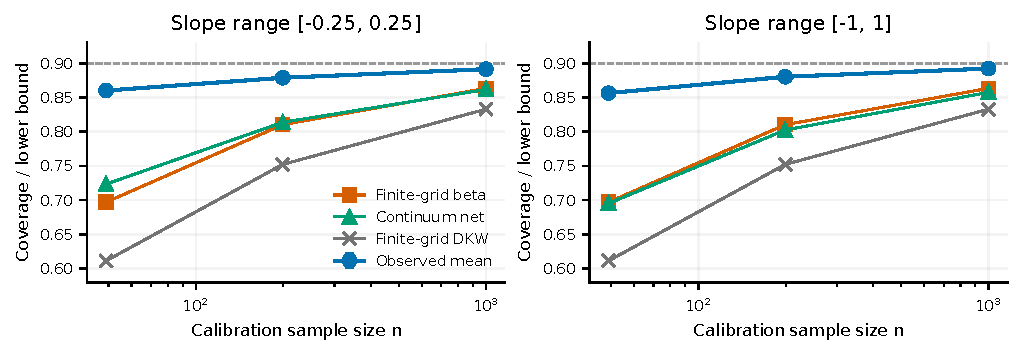
\includegraphics[width=\textwidth]{figures/certificates.pdf}
\caption{How informative are the sufficient conditions? Observed means and 95\% Monte Carlo intervals are compared with three 95\%-confidence lower certificates for the regular linear score family. The dashed line is the analytic fixed-score target 0.9. These are different statistical objects: the curves compare guarantee conservatism, not three prediction algorithms. No certificate is uniformly best.}
\label{fig:certificates}
\end{figure*}

Observed mean coverage ranged from 0.85636 at $n=49,a=1$ to 0.89225 at $n=999,a=1$, approaching the fixed-score target 0.9. The continuum certificate ranges from 0.69526 to 0.86162. It is sometimes stronger and sometimes weaker than the finite-grid beta certificate; for example at $n=999,a=1$ it is 0.85755 versus 0.86333. Both are stronger than the reported DKW certificate in these settings. The empirical fraction of calibration samples below the continuum lower certificate is between 0.001 and 0.003, well below 0.05, showing conservatism in this example rather than tightness. These finite simulations neither prove the bounds nor establish their utility for unknown distributions.

\paragraph{Implementation and cost.}
Eight verification tests cover quantile boundaries, all masks through $K=6$, exact rational occupancy enumeration, direct predictions and scale invariance, independent CDF quadrature, the beta/binomial identity, tiny nonzero slopes and infinite-threshold execution. They pass. Review exposed cancellation and an unhandled boundary outside the reported linear settings; both were fixed. Rerunning the unchanged protocol altered saved outcomes by at most $9.6\times10^{-15}$. The original confirmatory script ran in \RunSeconds{} seconds on an Apple M4 Max CPU with Python 3.12.12; this excludes setup and document preparation. No efficiency comparison or GPU computation is claimed. For large $K$, the code evaluates subset membership and uniform order statistics directly; it does not numerically optimize or store all the scalar knots.

\section{Limitations and Implications}

The negative example is designed to expose a missing assumption. It contains no informative predictor, encodes exponentially many subsets, and needs increasingly fine parameter precision. It supplies no evidence that normal temperature scaling, standard neural adapters, or ordinary hyperparameter grids exhibit near-zero coverage. The observations in \citet{zeng2025} can hold for their particular classes even though a general dimension-only theorem requires additional assumptions.

The positive result is a sufficient condition for coverage, not an efficient conformal algorithm. Population rank covers and uniform concentration bounds are typically unknown. Sup-norm covers can also be large or infinite in useful problems, while valid methods based on different arguments may still exist. The beta union bound ignores dependence between representatives and can be conservative. Ties, non-i.i.d. data and data-dependent score families without independent training are outside the stated results. Although raw scores are smooth in the construction, the selection objective is deliberately combinatorial.

The precise practical lesson is to justify calibration reuse using the actual threshold class, a valid selection-aware procedure, independent recalibration, or an appropriate stability argument. Merely counting tunable coordinates or reporting a small raw-score derivative does not supply such a justification. Determining whether the specific strengthened counterexample and synthesis warrant a full conference contribution requires external expert assessment.

\section{Conclusion}

Smooth scalar score tuning can cause arbitrarily severe finite-sample split-conformal coverage loss across a class of families, with an exact occupancy law in a simple construction. Classical uniform convergence nevertheless ensures consistency for each fixed compact bounded continuous family with atomless scores. Probability-scale covers make this distinction explicit and combine with classical beta tails to give a finite-sample certificate. Establishing tractable, data-driven estimates of the relevant complexity remains open.

\section*{Impact Statement}
This work concerns the reliability of uncertainty guarantees. A potential benefit is preventing unjustified calibration-data reuse. A potential misuse is to interpret a deliberately adversarial construction as evidence that all low-dimensional calibration fails, or to treat an oracle certificate with estimated constants as automatically valid. We explicitly limit both interpretations. Experiments use synthetic data only. No personal data, human participants, or deployed decision system is involved.

\section*{Research Process Disclosure}
This local draft was developed with autonomous AI assistance for literature search, derivations, implementation, writing and adversarial review. It has not been submitted or externally peer reviewed. Responsible human authorship and domain-expert verification are required before submission. The 2027 submission rules were unavailable at the audit date; the official 2026 template is used provisionally. The accompanying audit records distinguish generated hypotheses, executed checks and unresolved questions.

\bibliography{references}
\bibliographystyle{icml2026}

\newpage
\appendix
\onecolumn
\section{Smoothness and Score Distributions}\label{app:smooth}

Write $b_j(y)=\ind\{y\notin A_j\}$. On the interval $[\lambda_j,\lambda_{j+1}]$, the full score definition is
\begin{equation}
 S_\lambda(u,y)=a_K\left[b_j(y)+(b_{j+1}(y)-b_j(y))h((M-1)\lambda-j)+u/4\right].
\end{equation}
At the final endpoint, use the value at the last knot. The map $\psi$ is infinitely differentiable with every derivative zero at zero from the right. Therefore $h$ has zero derivatives of every positive order at both endpoints; adjacent interpolation pieces and the constant exterior extensions have matching derivatives of all orders. Since their unscaled values lie in $[0,5/4]$ and $a_K\le1/8$, scores lie in $[0,5/32]\subset[0,1]$.

For $0<t<1$, let $g(t)=1/(1-t)-1/t$. Then $h(t)=\operatorname{logistic}(g(t))$ and
\begin{equation}
 h'(t)=h(t)(1-h(t))\left(t^{-2}+(1-t)^{-2}\right).
\end{equation}
For $t\le1/2$, $g(t)\le2-1/t$, and $h(t)(1-h(t))\le e^{g(t)}$. Putting $v=1/t\ge2$ gives
\begin{equation}
 h'(t)\le e^2 e^{-v}(v^2+4)\le8,
\end{equation}
because $e^{-v}(v^2+4)$ is decreasing on $[2,\infty)$. Symmetry handles $t\ge1/2$. Multiplication by $a_K(M-1)$ proves the uniform derivative bound one. For each fixed $\lambda$, the score law is a mixture of $K$ uniform distributions, all of width $a_K/4$. It is atomless, with density bounded by $4/a_K$. This bound is finite for each fixed family but grows exponentially with $K$; atomlessness is not a uniform anti-concentration rate across families.

For completeness, when $K=1$ the score construction still applies with $M=2$, and the selected subset contains the sole label. The occupancy formula reduces to $c_n$. If $k=n+1$, all labels are included by the $+\infty$ convention and the occupancy formula is not used.

\section{Additional Details for the Consistency Result}\label{app:consistency}

We make the compactness step explicit. If $\omega(w)\not\to0$, choose $\eta>0$, $w_j\downarrow0$, parameters $\lambda_j$ and intervals $(t_j,t_j+w_j]$ with probability at least $\eta$. Since scores lie in $[0,1]$, only interval locations in a bounded region can have positive probability for small $w_j$. Pass to a subsequence with $\lambda_j\to\lambda_*$ and $t_j\to t_*$. On the interval event,
\begin{equation}
 |S_{\lambda_*}(Z)-t_*|\le L\|\lambda_j-\lambda_*\|+w_j+|t_j-t_*|=:e_j\to0.
\end{equation}
For any fixed $e>0$, all sufficiently large $j$ imply $\PP(|S_{\lambda_*}(Z)-t_*|\le e)\ge\eta$. Letting $e\downarrow0$ gives an atom of mass at least $\eta$, a contradiction.

Thus for any $r>0$, a sufficiently small parameter radius gives a rank net with error at most $r$. Its cardinality is finite and does not depend on $n$. For every center, the beta mean is $c_n\to1-\alpha$ and its variance is $k(n+1-k)/[(n+1)^2(n+2)]\to0$. A union bound over this fixed finite set gives convergence of both its maximum and minimum order statistics. This justifies the bracket argument without requiring a rate for the concentration modulus. It also shows why allowing $K$ and therefore the score family to change with $n$ falls outside the corollary.

\paragraph{Direct classical reduction under weaker conditions.}
Let $\Lambda\subset\R^d$ be compact, the scores bounded in $[0,1]$ and measurable, and suppose that at every fixed $\lambda$, $S_\mu(Z)\to S_\lambda(Z)$ almost surely as $\mu\to\lambda$. Assume $F_\lambda$ is continuous for every $\lambda$. On the compact index set $\Lambda\times[-1,2]$, consider $a(z,(\lambda,t))=\ind\{S_\lambda(z)\le t\}$. At each fixed $(\lambda,t)$ it is almost surely continuous in its index: the only possible obstruction is $S_\lambda(Z)=t$, which has probability zero. Its envelope is one. Lemma 2.4 of \citet{newey1994} therefore implies
\begin{equation}
 \Delta_n:=\sup_{\lambda,t}|F_{n,\lambda}(t)-F_\lambda(t)|\longrightarrow0
\end{equation}
in outer probability. At the selected $k$th order statistic, $F_{n,\hat\lambda}(q)\ge k/n$ and $F_{n,\hat\lambda}(q^-)\le(k-1)/n$. Continuity of the population CDF, including for every possible selected parameter, yields
\begin{equation}
 k/n-\Delta_n\le V_D\le(k-1)/n+\Delta_n.
\end{equation}
These inequalities allow calibration ties induced by selection. They imply the claimed convergence; since the selected coverage is measurable, its convergence is ordinary convergence in probability. This explicit reduction is prior-theory attribution, not an additional new theorem. It also shows that the Lipschitz assumption is useful for the quantitative transfer in \cref{eq:transfer}, while being stronger than needed for qualitative consistency.

\section{Implementation and Evaluation Details}\label{app:implementation}

The package contains \texttt{src/core.py}, the frozen configuration, raw compressed arrays, result tables, a reproduction script, and a Git history. Each raw row corresponds to an independently generated calibration sample. The occupancy files contain adaptive, fixed, split and monotone conditional coverage, the number of distinct labels, the uniform order statistic and the split threshold. The split control evaluates the exact CDF
\begin{equation}
 F_A(q)=p_A[4q]_0^1+(1-p_A)[4(q-1)]_0^1,\qquad p_A=|A|/K,
\end{equation}
where $[x]_0^1=\min(1,\max(0,x))$. Its tuning set and calibration set are disjoint. The monotone control uses $g_D(u)=(1+\overline U)u+\min_iU_i$, evaluates the transformed quantile, and inverts $g_D$. No simulated test labels are used in choosing a score or certificate.

The linear-score CDF used for evaluation is, with $b=|\beta|>0$,
\begin{equation}
 F_\beta(q)=\frac{(q+b)_+^2-(q-b)_+^2-(q+b-1)_+^2+(q-b-1)_+^2}{4b}.
\end{equation}
For $b=0$, it is $[q]_0^1$. This formula follows by integrating $[q-\beta x]_0^1/2$ over $x\in[-1,1]$; independent numerical quadrature is a verification test. The conditional prediction set is $\{y\in[0,1]:y\le q-\beta x\}$, so the CDF is precisely its coverage.

For $G=257$ candidates the finite-grid beta lower bound is $B_{n,k}^{-1}(\delta/G)$. The DKW lower bound reported in the figure is
\begin{equation}
 \left[\frac{k}{n}-\sqrt{\frac{\log(2G/\delta)}{2n}}\right]_+.
\end{equation}
The factor two comes from using the two-sided DKW inequality; sharper one-sided versions are possible. We do not claim optimality of this baseline. The continuum net lower bound maximizes
\begin{equation}
 \left[B_{n,k}^{-1}\left(\frac{\delta}{\lceil a/\epsilon\rceil+1}\right)-2\epsilon\right]_+
\end{equation}
over 2,000 fixed logarithmically spaced radii between $10^{-5}$ and $0.25$. A grid of that cardinality has spacing at most $2\epsilon$ over $[-a,a]$, and hence covering radius at most $\epsilon$. Radius choice depends on known analytical constants, not simulation outcomes. All certificates are single-setting 95\% probability statements; they are not a joint 95\% statement over all experimental settings.

\begin{figure}[h]
\centering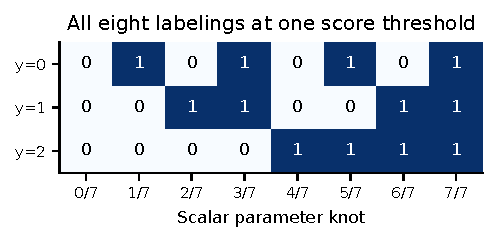
\includegraphics[width=.48\textwidth]{figures/shattering.pdf}
\caption{Executed exhaustive check for $K=3$. At $u=1/2$ and the common threshold $a_K/2$, the smooth scalar knots realize every binary membership vector. This directly refutes a VC-dimension upper bound of two under only bounded continuous scalar parameterization.}
\end{figure}

Floating-point evaluation of the explicit scalar interpolation is restricted to $K\le20$ in the code. Tests use up to $K=12$, with exhaustive masks through $K=6$. Larger simulations operate on the mathematical identity in \cref{eq:conditional-occupancy} and independently audit its prediction event. A mask array does not instantiate the large-precision scalar; this is an exact alternative representation for checking the probability calculation. No claim about the numerical stability of huge scalar parameterizations follows.

\section{Full Confirmatory Results}\label{app:full}

The following entries were all specified before confirmatory execution. Main-run seed: 73190421, with deterministic child streams by case index. The regular-family seed is 972041; the independent-test audit seed is 971144. Pilot seed: 20260928. Confidence intervals are pointwise mean $\pm1.96$ empirical standard error across repetitions. They measure numerical Monte Carlo precision, not uncertainty about the validity of a proved identity. Every occupancy case uses 10,000 repetitions and every linear case uses 1,000.

\begin{table}[h]
\centering\small
\caption{Full occupancy results, in percent. Monotone control equals the fixed control up to floating-point roundoff and is preserved in the raw data.}
\begin{tabular}{rrrrrrr}
\toprule
$n$ & $K$ & $\alpha$ & Exact adaptive & Adaptive & Fixed & Disjoint split \\
\midrule
\inputtable{generated/all_occupancy_table.tex}
\bottomrule
\end{tabular}
\end{table}

\begin{table}[h]
\centering\small
\caption{Linear family. Observed coverage and lower certificates are in percent. The final column counts calibration samples below the continuum certificate out of 1,000.}
\begin{tabular}{rrrrrrr}
\toprule
$n$ & $a$ & Observed coverage (\%) & Grid beta & Continuum & DKW & Below continuum \\
\midrule
\inputtable{generated/linear_table.tex}
\bottomrule
\end{tabular}
\end{table}

\section{Scope of Verification and Reproduction}

The automated checks validate implementations and finite examples. The mathematical arguments were written and adversarially checked with AI assistance; no claim of independent human verification is made. No actual deep-learning benchmark, training run, ImageNet replication, or experiment on a practical temperature scaler was conducted. The public official implementation of the closest ICML paper was inspected for intended scope only.

The reference audit records which version and sections were inspected for every citation. Three cited 2026 works are preprints, not treated as peer-reviewed validation. The audit searched for corrections and closely related counterexamples; absence from the search is not proof of novelty. A concise contribution statement, claim-to-evidence map, review passes, issue table and remaining research questions are provided separately from the manuscript. Nothing in this local package constitutes submission, publication or acceptance.

\end{document}
